\begin{enumerate}

%%%%%%%%% Problem 1 %%%%%%%%%%%
\item Create the DEPT table based on the following table instance chart. Place the
syntax in a script called \texttt{lab9\_1.sql}, then execute the statement in the script to create the table.
Confirm that the table is created
\begin{figure}[h]
\centering
    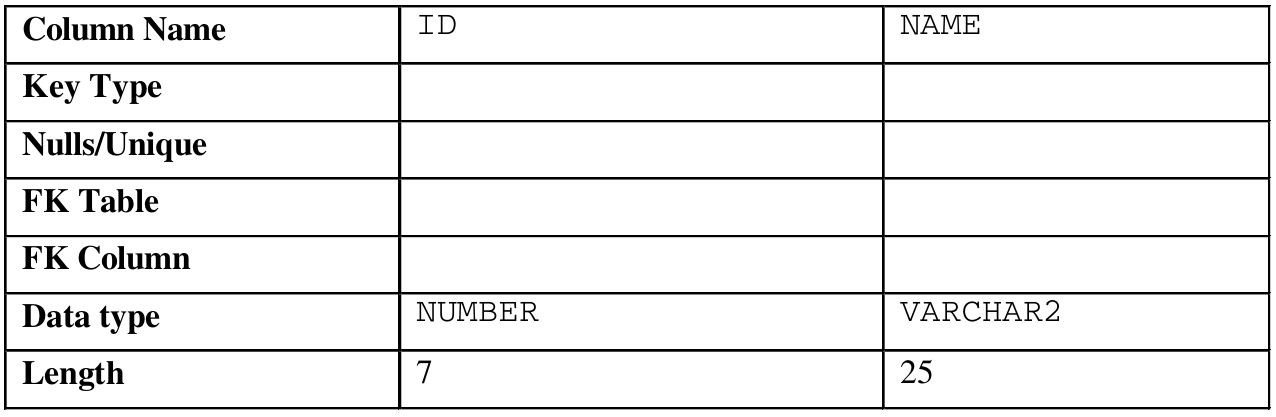
\includegraphics[width=.7\linewidth]{graphics/91.png}
\end{figure}

\textbf{Solution: }
\begin{lstlisting}[language=SQL]
CREATE TABLE dept(
    id NUMBER(7),
    name VARCHAR2(25)
);
DESCRIBE DEPT;
\end{lstlisting}
\textbf{Output: }
\begin{figure}[h]
    \centering
    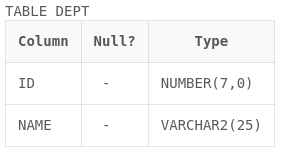
\includegraphics[width=0.5\linewidth]{graphics/p91.png}
\end{figure}

%%%%%%%%% Problem 2 %%%%%%%%%%%
\item Populate the DEPT table with data from the DEPARTMENTS table. Include only columns that
you need.

\textbf{Solution: }
\begin{lstlisting}[language=SQL]
INSERT INTO dept
SELECT department_id, department_name
FROM hr.departments;
\end{lstlisting}

%%%%%%%%% Problem 3 %%%%%%%%%%%
\item Create the EMP table based on the following table instance chart. Place the syntax in a script called
\texttt{lab9\_3.sql}, and then execute the statement in the script to create the table. Confirm that the table is
created.
\begin{figure}[h]
\centering
    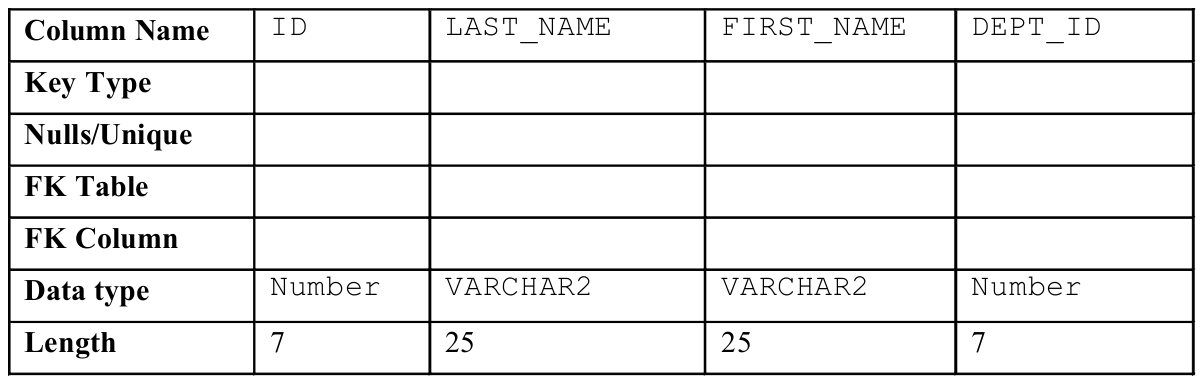
\includegraphics[width=.7\linewidth]{graphics/93.png}
\end{figure}

\textbf{Solution: }
\begin{lstlisting}[language=SQL]
CREATE TABLE emp(
    id number (7),
    last_name varchar2(25),
    first_name varchar2(25),
    dept_id number (7)
);

DESCRIBE emp;
\end{lstlisting}
\textbf{Output: }
\begin{figure}[h]
    \centering
    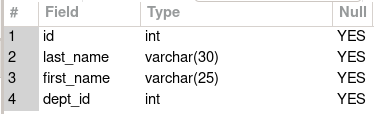
\includegraphics[width=0.4\linewidth]{graphics/p93.png}
\end{figure}

%%%%%%%%% Problem 4 %%%%%%%%%%%
\item Modify the EMP table to allow for longer employee last names. Confirm your modification.
\begin{figure}[h]
\centering
    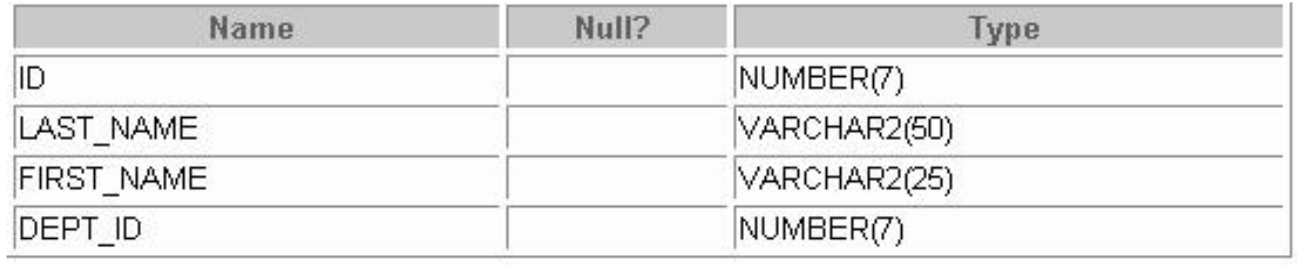
\includegraphics[width=.7\linewidth]{graphics/94.png}
\end{figure}

\textbf{Solution: }
\begin{lstlisting}[language=SQL]
ALTER TABLE emp
MODIFY (last_name VARCHAR2(50));
DESCRIBE emp;
\end{lstlisting}

\textbf{Output: }
\begin{figure}[h]
    \centering
    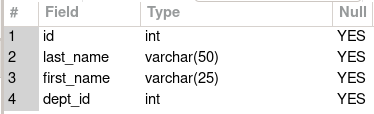
\includegraphics[width=0.35\linewidth]{graphics/p94.png}
\end{figure}

%%%%%%%%% Problem 5 %%%%%%%%%%%
\newpage
\item Confirm that both the DEPT and EMP tables are stored in the data dictionary. (Hint:
\texttt{USER\_TABLES})
\begin{figure}[h]
\centering
    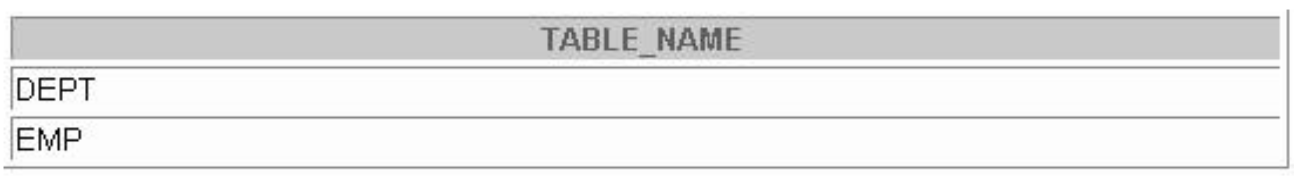
\includegraphics[width=.5\linewidth]{graphics/95.png}
\end{figure}

\textbf{Solution: }
\begin{lstlisting}[language=SQL]
select table_name
from user_tables
where table_name in ('DEPT','EMP');
\end{lstlisting}
\textbf{Output: }
\begin{figure}[h]
    \centering
    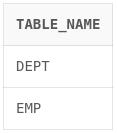
\includegraphics[width=0.2\linewidth]{graphics/p95.png}
\end{figure}

%%%%%%%%% Problem 6 %%%%%%%%%%%
\item Create the EMPLOYEES2 table based on the structure of the EMPLOYEES table. Include only the
EMPLOYEE\_ID, FIRST\_NAME, LAST\_NAME, SALARY, and DEPARTMENT\_ID columns. Name
the columns in your new table ID, FIRST\_NAME, LAST\_NAME, SALARY , and DEPT\_ID,
respectively.

\textbf{Solution: }
\begin{lstlisting}[language=SQL]
CREATE TABLE employees2 AS
SELECT employee_id id, first_name, last_name, salary, 
    department_id dept_id
from hr.employees;
\end{lstlisting}

%%%%%%%%% Problem 7 %%%%%%%%%%%
\item Drop the EMP table.

\textbf{Solution: }
\begin{lstlisting}[language=SQL]
DROP TABLE emp;
\end{lstlisting}

%%%%%%%%% Problem 8 %%%%%%%%%%%
\item Rename the EMPLOYEES2 table as EMP.

\textbf{Solution: }
\begin{lstlisting}[language=SQL]
ALTER TABLE employees2 RENAME TO emp;
\end{lstlisting}

%%%%%%%%% Problem 9 %%%%%%%%%%%
\item Add a comment to the DEPT and EMP table definitions describing the tables. Confirm your
additions in the data dictionary.

\textbf{Solution: }
\begin{lstlisting}[language=SQL]
COMMENT ON TABLE emp IS 
    'This table stores employee information';
COMMENT ON TABLE dept IS 
    'This table stores dept information';
SELECT *
FROM user_tab_comments
WHERE table_name = 'DEPT'
	OR table_name = 'EMP';
\end{lstlisting}
\textbf{Output: }
\begin{figure}[h]
    \centering
    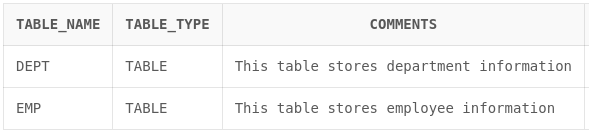
\includegraphics[width=0.8\linewidth]{graphics/p99.png}
\end{figure}

%%%%%%%%% Problem 10 %%%%%%%%%%%
\item Drop the \texttt{FIRST\_NAME} column from the EMP table. Confirm your modification by checking the
description of the table.

\textbf{Solution: }
\begin{lstlisting}[language=SQL]
ALTER TABLE emp
DROP COLUMN FIRST_NAME;
DESCRIBE emp;
\end{lstlisting}
\textbf{Output: }
\begin{figure}[h]
    \centering
    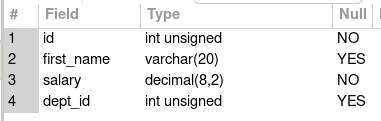
\includegraphics[width=0.5\linewidth]{graphics/p910.png}
\end{figure}

%%%%%%%%% Problem 11 %%%%%%%%%%%
\item In the EMP table, mark the \texttt{DEPT\_ID} column as UNUSED. Confirm your
modification by checking the description of the table.

\textbf{Solution: }
\begin{lstlisting}[language=SQL]
ALTER TABLE emp
SET UNUSED (dept_id);

DESCRIBE emp;
\end{lstlisting}
\textbf{Output: }
\begin{figure}[h]
    \centering
    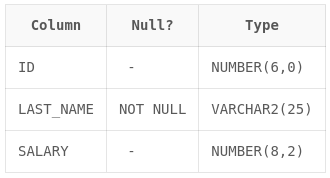
\includegraphics[width=0.5\linewidth]{graphics/p911.png}
\end{figure}
%%%%%%%%% Problem 12 %%%%%%%%%%%
\item Drop all the UNUSED columns from the EMP table. Confirm your modification by checking the
description of the table.

\textbf{Solution: }
\begin{lstlisting}[language=SQL]
ALTER TABLE emp
DROP UNUSED COLUMNS;

DESCRIBE emp;
\end{lstlisting}
\textbf{Output: }
\begin{figure}[h]
    \centering
    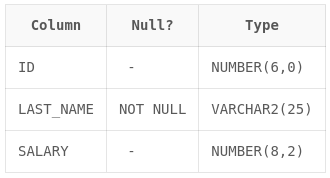
\includegraphics[width=0.5\linewidth]{graphics/p911.png}
\end{figure}
\end{enumerate}
